% ============================================================================================
% BAB III ANALISIS MASALAH
% Pembagian subbab tidak rigid dan dapat bervariasi. Bab ini minimal berisi analisis kebutuhan
% fungsional dan nonfungsional, analisis berbagai alternatif solusi yang dapat ditawarkan, dan
% metode pemilihan solusi yang diusulkan.
% ============================================================================================
\cleardoublepage
\chapter{ANALISIS MASALAH}
\label{chap:analisis-masalah}
% Bab ini membahas analisis masalah yang ada pada sistem saat ini, analisis kebutuhan yang diperlukan
% untuk menyelesaikan masalah tersebut, serta analisis pemilihan solusi yang diusulkan. Secara garis besar,
% bab ini membahas hal-hal berikut:
% \begin{enumerate}[1.]
%     \item Deskripsi hasil analisis dari persoalan yang sedang ditangani dalam TA;
%     \item Penjelasan tentang solusi yang ditawarkan (dapat berupa algoritma, konsep desain, formula, atau gabungannya) 
%     pada level konsep dan detail yang cukup untuk merealisasikan solusinya; dan
%     \item Penjelasan tentang pendekatan yang dipilih dalam menyelesaikan persoalan TA.
% \end{enumerate}
% Subbab-subbab dalam bab ini dapat disesuaikan dengan kebutuhan topik TA yang dibahas. Berikut adalah penjabaran analisis masalah dan kebutuhan untuk pengembangan sistem prediksi hipertensi.

\section{Analisis Kondisi Saat Ini}
Sistem deteksi dini hipertensi di Indonesia saat ini secara umum berjalan melalui dua jalur utama, yaitu skrining mandiri berbasis aplikasi dan pemeriksaan fisik berkala di fasilitas kesehatan. Keduanya dirancang untuk mendeteksi risiko penyakit sejak dini, sebelum kondisi berkembang menjadi komplikasi yang serius. Jalur pertama yaitu menggunakan fitur "Skrining Riwayat Kesehatan" pada aplikasi Mobile JKN yang dikelola oleh BPJS Kesehatan, sehingga peserta dapat menilai tingkat risikonya secara mandiri berdasarkan riwayat dan gaya hidup tanpa harus lebih dahulu datang ke fasilitas kesehatan. Jalur kedua berupa pengukuran dan pemeriksaan langsung oleh tenaga medis di Fasilitas Kesehatan Tingkat Pertama (FKTP). Subbab ini menganalisis kedua jalur tersebut sebagai kondisi awal (\emph{as-is}) untuk memahami keterbatasan proses yang berjalan saat ini, sekaligus menjadi dasar perumusan solusi yang diusulkan pada penelitian ini.

\subsection{Skrining Mandiri Berbasis Aplikasi: Skrining Riwayat Kesehatan pada Mobile JKN}
Jalur pertama deteksi dini merupakan skrining mandiri berbasis aplikasi melalui fitur Skrining Riwayat Kesehatan (SRK) pada aplikasi Mobile JKN yang dikelola oleh BPJS Kesehatan \autocite{Juwita2022SRK}. Fitur ini dirancang untuk mendeteksi potensi risiko penyakit tidak menular (PTM) sejak dini pada peserta Jaminan Kesehatan Nasional, dengan menyasar empat penyakit dengan beban tertinggi di Indonesia, yaitu diabetes melitus, hipertensi, penyakit ginjal kronis, dan penyakit jantung koroner \autocite{Juwita2022SRK}.

\begin{figure}[H]
    \centering
    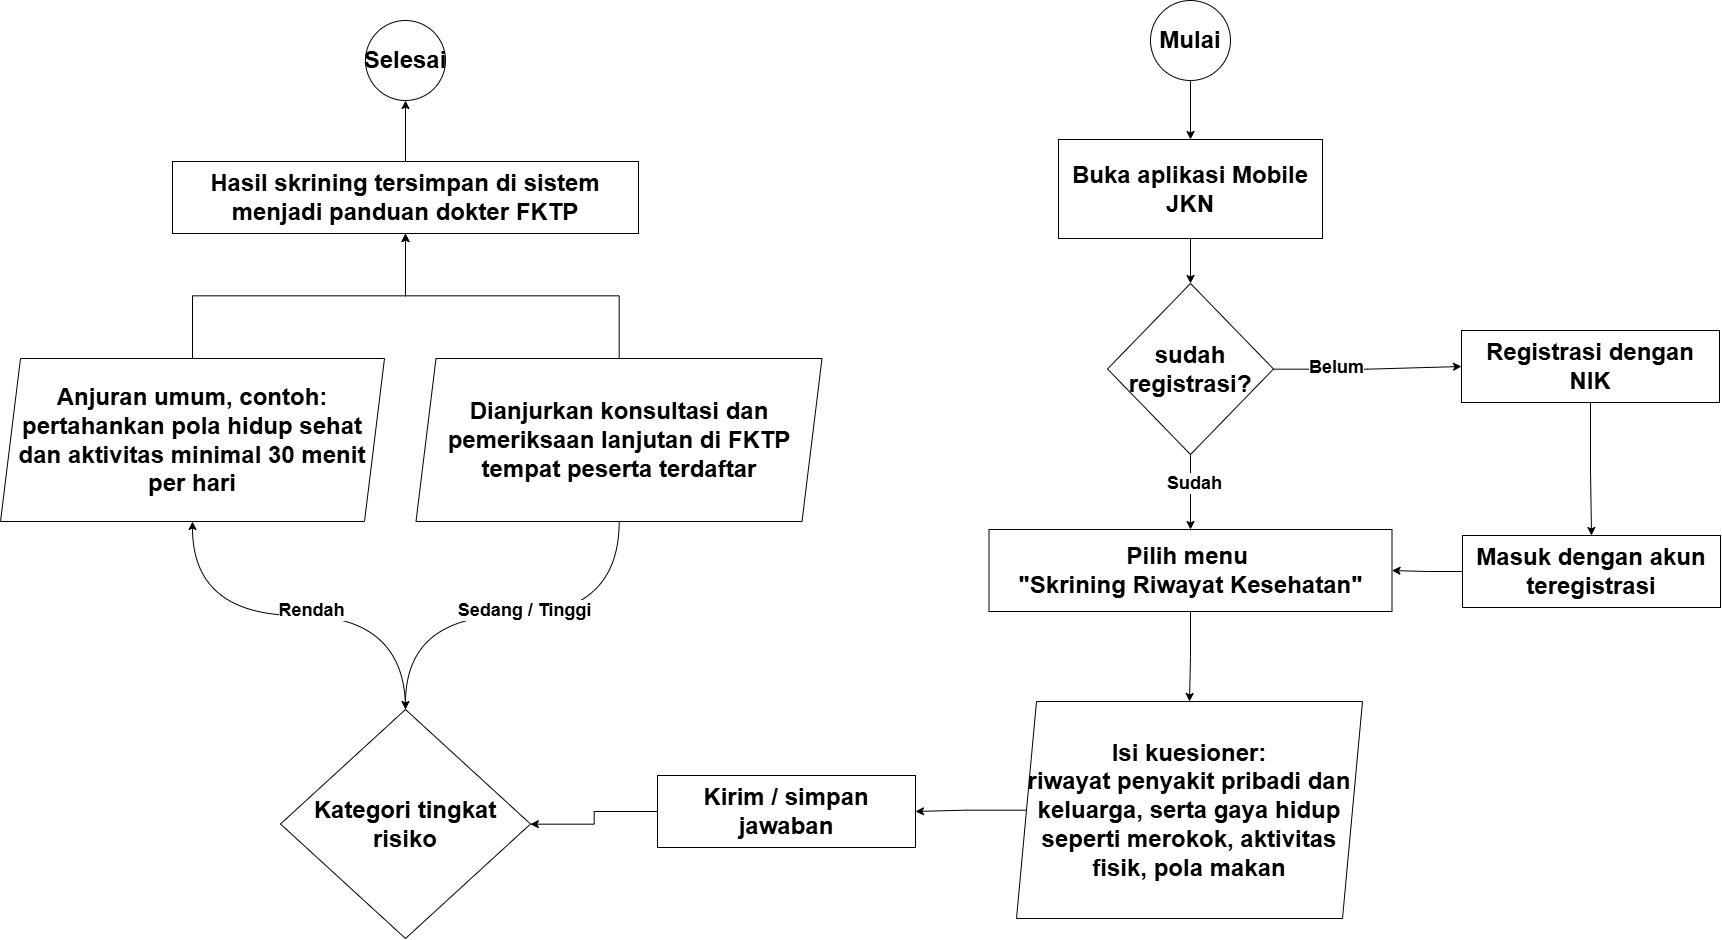
\includegraphics[width=0.9\textwidth]{images/Alur-skrining-MobileJKN.png}
    \caption{Alur mekanisme Skrining Riwayat Kesehatan (SRK) pada aplikasi Mobile JKN}
    \label{fig:alur-srk}
\end{figure}
Alur mekanisme kerja fitur Skrining Riwayat Kesehatan (SRK) pada aplikasi Mobile JKN ditunjukkan pada Gambar~\ref{fig:alur-srk}. Peserta masuk ke aplikasi Mobile JKN menggunakan Nomor Induk Kependudukan (NIK), kemudian memilih menu Skrining Riwayat Kesehatan dan menjawab sejumlah pertanyaan terstruktur mengenai gaya hidup harian serta riwayat penyakit pada diri sendiri maupun keluarga, seperti kebiasaan merokok, aktivitas fisik, pola makan, serta riwayat keluarga terhadap keempat penyakit tersebut. Berdasarkan jawaban tersebut, sistem menghitung dan mengeluarkan hasil berupa kategori tingkat risiko, yaitu risiko rendah, sedang, atau risiko tinggi, terhadap masing-masing penyakit. Hasil skrining ini kemudian tersimpan pada sistem dan menjadi panduan bagi dokter di FKTP tempat peserta terdaftar, peserta dengan hasil berisiko tinggi diarahkan untuk menindaklanjuti melalui pemeriksaan lebih lanjut di fasilitas kesehatan \autocite{Juwita2022SRK}.

Karakteristik penting dari jalur ini adalah penilaian risiko yang sepenuhnya bertumpu pada faktor risiko riwayat dan gaya hidup yang dilaporkan sendiri oleh peserta, bukan pada pengukuran tekanan darah langsung. Pendekatan berbasis faktor risiko non-laboratorium inilah yang menjadi konteks utama penelitian ini, karena memungkinkan estimasi risiko dilakukan lebih awal sebelum tekanan darah tinggi benar-benar terukur. Meskipun demikian, keluaran SRK saat ini berupa kategori tingkat risiko (rendah, sedang, atau tinggi) yang disertai anjuran umum, seperti menjaga pola hidup sehat atau berkonsultasi ke FKTP, tetapi belum menjelaskan secara personal faktor mana yang paling berkontribusi terhadap risiko masing-masing peserta. Dengan kata lain, hasil skrining menunjukkan seberapa besar risiko seseorang, tetapi belum menjelaskan mengapa risiko tersebut muncul, sehingga masih terdapat ruang untuk meningkatkan sifat personal dan nilai edukatif dari hasil skrining tersebut.

\subsection{Prosedur Skrining Hipertensi di Fasilitas Kesehatan Tingkat Pertama}
Jalur kedua deteksi dini berupa skrining dan pemeriksaan hipertensi di Fasilitas Kesehatan Tingkat Pertama (FKTP), yang saat ini masih bergantung pada pengukuran klinis konvensional dan penilaian manual oleh tenaga medis. Pasien yang datang ke FKTP menjalani proses registrasi terlebih dahulu, kemudian perawat melakukan anamnesis serta pengukuran antropometri dan tekanan darah (TD), meliputi tinggi badan, berat badan, lingkar perut, dan tensi. Apabila tekanan darah melampaui ambang 140/90 mmHg, dokter melanjutkan dengan analisis hasil dan menilai faktor risiko pasien, seperti usia, status merokok, dan kadar gula darah, untuk menentukan status kesehatan serta tata laksananya sebagaimana digambarkan pada Gambar~\ref{fig:alur-konvensional}.

Jalur ini efektif untuk menegakkan diagnosis secara akurat, tetapi mensyaratkan kehadiran fisik pasien di fasilitas kesehatan. Ketergantungan pada kehadiran fisik inilah yang menjadi salah satu penyebab cakupan deteksi dini hipertensi belum optimal, baik secara global \autocite{Mills2020Global} maupun di Indonesia, dengan sebagian besar penderita belum terdiagnosis dan baru menyadari kondisinya setelah timbul komplikasi \autocite{ri2018}. Hambatan akses turut memperberat kondisi ini, salah satunya beban antrean dan waktu tunggu yang panjang di Puskesmas; sebuah studi di layanan rawat jalan Puskesmas mencatat 93,5\% pasien mengalami waktu tunggu lebih dari 60 menit \autocite{Manyering2023}, kondisi yang dapat menurunkan kenyamanan dan menjadi disinsentif bagi masyarakat untuk memeriksakan diri secara rutin.

Kondisi tersebut menunjukkan bahwa skrining yang sepenuhnya bergantung pada kehadiran fisik di FKTP belum memadai untuk mendorong deteksi dini secara luas. Diperlukan jalur skrining awal yang dapat diakses secara mandiri agar masyarakat lebih dahulu menyadari tingkat risikonya, sehingga kesadaran tersebut dapat mengarahkan mereka untuk menjalani pemeriksaan lanjutan di fasilitas kesehatan secara lebih tepat sasaran.

Selain hambatan akses tersebut, keterbatasan waktu konsultasi dan kompleksitas interaksi antar faktor risiko membuat penilaian risiko secara manual sulit dilakukan secara komprehensif untuk setiap pasien. Keterbatasan inilah yang mendorong tren pemanfaatan algoritma \textit{machine learning} sebagai alat bantu prediksi risiko yang lebih dini dan akurat. Namun, penerapan model ML konvensional, seperti Neural Networks atau Ensemble Trees, sering kali menghadapi kendala transparansi. Model tersebut bekerja sebagai kotak hitam atau biasa disebut juga dengan \textit{black box}, memberikan skor risiko tanpa disertai alasan medis yang jelas. Kondisi ini menciptakan keraguan di kalangan praktisi medis untuk mengadopsi hasil prediksi komputer dalam pengambilan keputusan klinis \autocite{Amann2020Explainability}.

\begin{figure}[H]
    \centering
    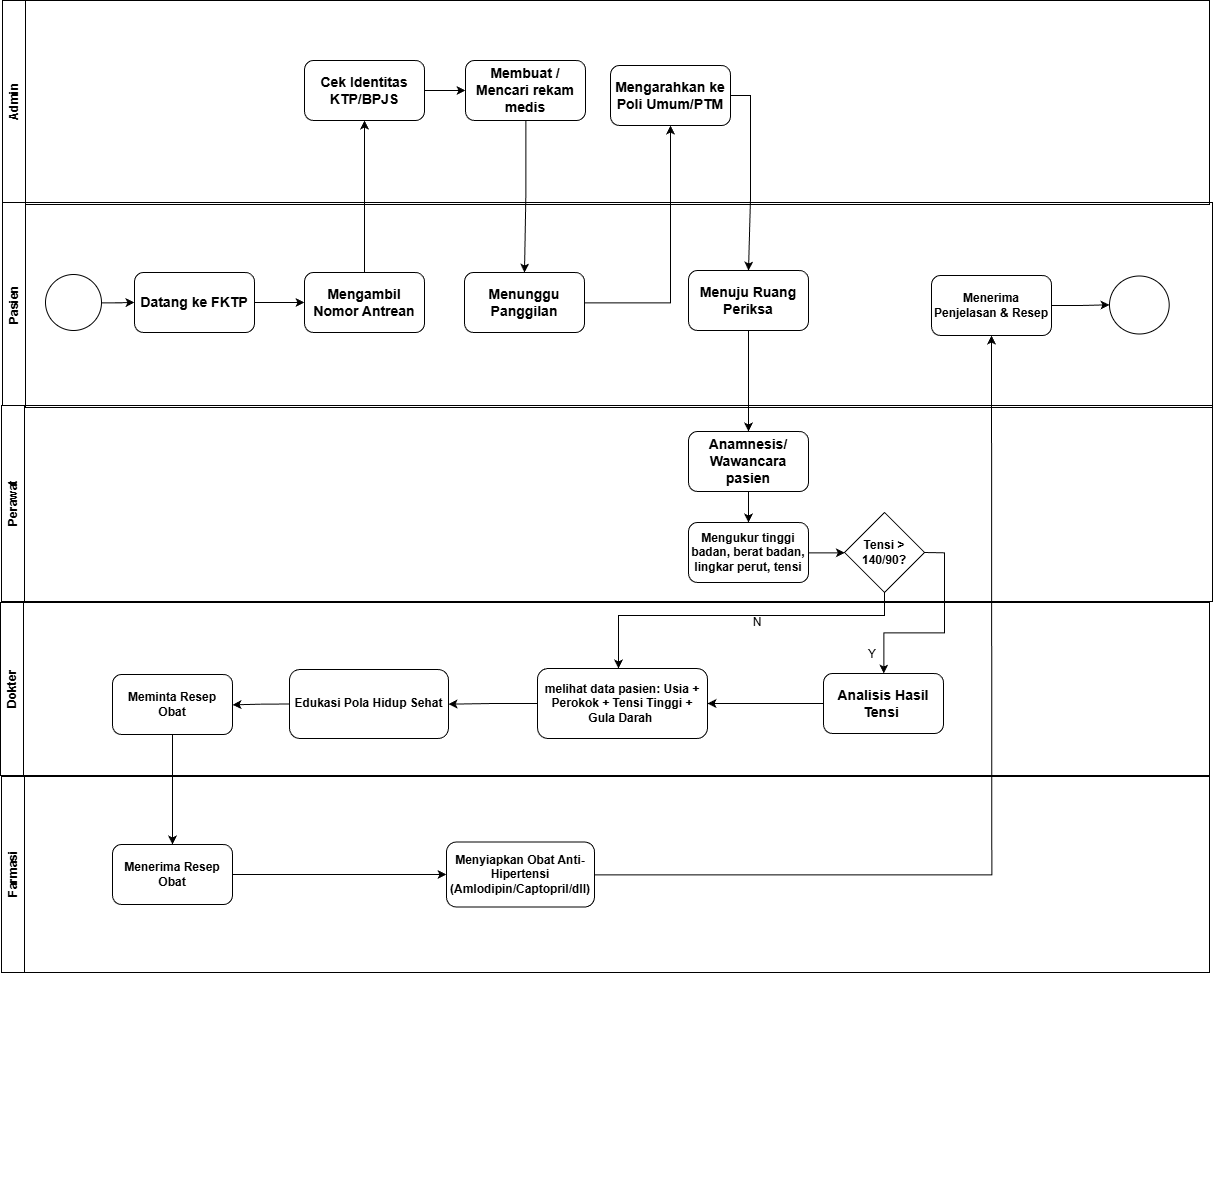
\includegraphics[width=0.9\textwidth]{images/gambar1.png}
    \caption{Alur skrining hipertensi di Fasilitas Kesehatan Tingkat Pertama (FKTP)}
    \label{fig:alur-konvensional}
\end{figure}

\subsection{Pemanfaatan Teknologi Prediksi Berbasis AI dan Keterbatasannya}
Untuk mengatasi keterbatasan tersebut, penelitian terkini mulai memanfaatkan teknologi prediksi berbasis kecerdasan artifisial. Salah satu arah utamanya adalah integrasi Explainable Artificial Intelligence (XAI) untuk membuka mekanisme model prediksi yang bersifat \textit{black box}. Meskipun demikian, luaran dari XAI umumnya masih berupa grafik fitur atau nilai matematis yang sulit dipahami oleh pasien awam. Kesenjangan komunikasi ini menjadi tantangan baru dalam menyampaikan risiko kesehatan kepada pasien secara efektif. Di sisi lain, kemunculan Large Language Model (LLM) menawarkan potensi untuk menarasikan data tersebut, namun penggunaannya yang tanpa pengawasan rentan menghasilkan informasi yang tidak valid atau halusinasi medis \autocite{Clusmann2023Future}. Oleh karena itu, kondisi saat ini menunjukkan adanya fragmentasi antara kemampuan prediksi yang tinggi, kebutuhan akan transparansi (\emph{explainability}), dan penyajian informasi yang akurat secara medis.

\subsection{Kesenjangan Transparansi dan Kepercayaan Klinis}
Masalah paling fundamental dalam adopsi teknologi prediksi risiko saat ini terletak pada kesenjangan pemahaman antara cara kerja model komputasi dan logika klinis dokter. Model \textit{machine learning} yang memiliki performa akurasi tinggi sering kali memiliki struktur internal yang sangat kompleks dan tidak dapat ditafsirkan secara langsung. Hal ini menciptakan dua hambatan utama dalam implementasi klinis:

\begin{enumerate}
    \item \textbf{Skeptisisme Tenaga Medis}\\
    Dokter dan tenaga kesehatan memegang tanggung jawab etis dan hukum atas keputusan yang diambil. Mereka enggan menggunakan prediksi dari sistem yang tidak dapat menjelaskan "mengapa" seorang pasien dikategorikan berisiko tinggi, terutama jika prediksi tersebut bertentangan dengan intuisi klinis mereka. Ketiadaan kausalitas yang dapat diobservasi menyebabkan rendahnya tingkat kepercayaan terhadap sistem pendukung keputusan berbasis AI \autocite{Linardatos2021Explainable}.
    
    \item \textbf{Kebingungan Pasien terhadap Hasil Prediksi}\\
    Bagi pasien, menerima diagnosis atau prediksi risiko tanpa penjelasan yang personal dapat menimbulkan kecemasan atau justru penyangkalan. Pasien membutuhkan narasi yang menghubungkan gaya hidup mereka (misalnya, merokok atau IMT tinggi) dengan kenaikan risiko yang diprediksi, bukan sekadar angka probabilitas statistik. Tanpa penjelasan yang memadai, kepatuhan pasien terhadap saran preventif cenderung rendah.
\end{enumerate}

\subsection{Risiko Halusinasi dan Inkonsistensi Informasi Medis}
Dari perspektif teknologi Generative AI yang mulai marak digunakan, tantangannya bersifat validitas data. Meskipun LLM mampu menghasilkan teks yang sangat koheren dan menyerupai bahasa manusia, model ini memiliki kecenderungan inheren untuk menghasilkan fakta yang salah atau "berhalusinasi" ketika tidak memiliki konteks yang cukup. Dalam domain medis yang berisiko tinggi, hal ini menciptakan bahaya laten sebagai berikut:

\begin{enumerate}
    \item Misinformasi Saran Medis\\
    Tanpa batasan basis pengetahuan yang ketat, LLM dapat memberikan saran kesehatan yang terlihat meyakinkan namun tidak memiliki dasar ilmiah atau bertentangan dengan pedoman medis resmi. Misalnya, model mungkin menyarankan dosis obat atau interpretasi gejala yang salah \autocite{Li2023ChatGPT}. Hal ini sangat berbahaya jika dijadikan rujukan oleh pengguna awam tanpa verifikasi.
    
    \item Inkonsistensi Narasi\\
    Penjelasan yang dihasilkan oleh model bahasa standar dapat bervariasi secara signifikan meskipun diberikan input data yang sama pada waktu yang berbeda. Ketidakkonsistenan ini mengurangi reliabilitas sistem sebagai alat edukasi pasien yang terstandarisasi. Tidak adanya mekanisme validasi silang (\emph{cross-validation}) dengan dokumen medis terpercaya membuat luaran model sulit dipertanggungjawabkan \autocite{Ji2023Survey}.
\end{enumerate}

\subsection{Tantangan Kompleksitas Data Multidimensi}
Pada konteks teknis pengolahan data, masalah diperparah dengan sifat data kesehatan yang heterogen dan non-linier. Faktor risiko hipertensi melibatkan interaksi yang rumit antara demografi, tanda vital, dan riwayat gaya hidup yang tidak selalu dapat dimodelkan dengan regresi linier sederhana.
\begin{enumerate}
    \item \textbf{Interaksi Variabel yang Tersembunyi}\\
    Metode statistik tradisional sering gagal menangkap hubungan non-linier yang kompleks, misalnya bagaimana dampak indeks massa tubuh (IMT) terhadap tekanan darah mungkin berbeda secara drastis tergantung pada usia dan tingkat aktivitas fisik seseorang. Kegagalan menangkap nuansa ini menyebabkan prediksi menjadi kurang akurat untuk individu dengan profil risiko yang unik \autocite{Elshawi2019Interpretability}.
    
    \item \textbf{Keterbatasan Personalisasi}\\
    Sistem informasi kesehatan yang ada saat ini umumnya bersifat \emph{one-size-fits-all} atau satu ukur untuk semua. Belum tersedia mekanisme yang secara otomatis mengadaptasi penjelasan risiko berdasarkan profil spesifik pasien secara \emph{real-time} yang didukung oleh bukti literatur medis terkini.
\end{enumerate}

\subsection{Identifikasi Kesenjangan (Gap Analysis)}
Berdasarkan analisis kondisi saat ini, dilakukan pemetaan kesenjangan antara kondisi \emph{As-Is} (sistem konvensional/\textit{black box}) dengan kondisi ideal \emph{To-Be} (sistem yang diusulkan) yang dirangkum dalam Tabel \ref{tab:gap-analysis} di bawah ini.

\begin{table}[H]
    \caption{Identifikasi Kesenjangan (Gap Analysis)}
    \label{tab:gap-analysis}
    \centering
    \small
    \begin{tabular}{|p{2.5cm}|p{3.5cm}|p{3.5cm}|p{3.5cm}|}
        \hline
        \textbf{Domain Masalah} & \textbf{Kondisi Saat Ini (\emph{As-Is})} & \textbf{Kesenjangan (Gap)} & \textbf{Kondisi Ideal (\emph{To-Be})} \\
        \hline
        Transparansi \& Kepercayaan & Model prediksi bekerja sebagai \textit{black box}; pengguna hanya menerima skor risiko tanpa alasan penjelas. & Tidak adanya mekanisme untuk menelusuri alasan di balik prediksi dominan variabel. & Sistem menyediakan fitur visualisasi (XAI) yang menjelaskan variabel dominan penyebab risiko. \\
        \hline
        Validitas Informasi & Penjelasan risiko jika menggunakan LLM biasa masih rentan terhadap halusinasi dan tidak memiliki referensi yang jelas. & Risiko kesalahan informasi medis yang membahayakan keselamatan pasien. & Narasi penjelasan dikendalikan melalui kombinasi kaidah deterministik dan \textit{prompt engineering} (\emph{guardrail}); angka dan arah pengaruh ditetapkan secara deterministik dari kontribusi faktor risiko yang dihasilkan metode XAI sehingga LLM tidak mengarang klaim medis di luar fakta sistem. \\
        \hline
        Akurasi \& Personalisasi & Analisis risiko bersifat reaktif dan generalis; sering mengabaikan interaksi non-linier antar variabel. & Rendahnya sensitivitas terhadap profil risiko individu dan kurangnya personalisasi. & Model ML mampu menangkap pola kompleks dan menyajikan narasi personal yang mudah dipahami awam. \\
        \hline
    \end{tabular}
\end{table}

Analisis kesenjangan pada Tabel \ref{tab:gap-analysis} menggarisbawahi bahwa tantangan yang dihadapi tidak hanya sekadar meningkatkan akurasi angka prediksi, tetapi juga membangun jembatan komunikasi antara logika mesin dan pemahaman manusia. Secara kumulatif, kesenjangan ini menegaskan urgensi pengembangan sistem terintegrasi yang menggabungkan kekuatan prediksi \textit{machine learning}, transparansi XAI, dan kemampuan naratif LLM yang dikendalikan melalui prompt engineering. Untuk mewujudkan solusi tersebut, langkah selanjutnya adalah menerjemahkan temuan ini ke dalam analisis kebutuhan sistem yang terukur.

\section{Analisis Kebutuhan}
Dalam perancangan sistem pendukung keputusan klinis yang menggabungkan kecerdasan buatan dan interpretasi bahasa alami ini, diperlukan pemahaman mendalam terhadap kebutuhan pengguna serta spesifikasi teknis yang ketat. Mengingat domain kesehatan merupakan area yang sensitif terhadap keselamatan (\emph{safety-critical}), analisis kebutuhan tidak cuma bergantung pada akurasi komputasi, namun juga pada aspek kepercayaan, transparansi, dan validitas informasi yang disampaikan kepada pengguna \autocite{Amann2020Explainability}. Tahapan ini bertujuan menerjemahkan kesenjangan masalah yang telah diidentifikasi sebelumnya menjadi spesifikasi fungsional dan non-fungsional yang terukur.

\subsection{Identifikasi Masalah Pengguna}
Pengguna utama sistem ini adalah masyarakat umum sebagai penerima informasi hasil skrining dan edukasi kesehatan. Di samping itu, tenaga medis profesional diposisikan sebagai pihak yang meninjau dan memvalidasi kelayakan keluaran sistem (\emph{validator}), sehingga kebutuhan akan transparansi dari sudut pandang medis tetap menjadi pertimbangan penting dalam perancangan. Masalah spesifik yang mendasari kebutuhan sistem dari kedua sudut pandang tersebut adalah sebagai berikut:

\begin{enumerate}
    \item Masyarakat Umum/Pasien\\
    Tantangan utama yang dihadapi pasien adalah ketidakmampuan untuk memahami terminologi medis yang kompleks dan angka probabilitas statistik yang dihasilkan oleh alat kesehatan konvensional. Pasien sering kali menerima hasil diagnosis atau prediksi risiko tanpa penjelasan kausalitas yang memadai mengenai faktor gaya hidup apa yang memicu risiko tersebut \autocite{Adadi2018}. Selain itu, kurangnya akses terhadap informasi kesehatan yang terpersonalisasi membuat pasien kesulitan menentukan langkah mitigasi mandiri yang tepat tanpa harus berkonsultasi panjang dengan dokter.
    
    \item Tenaga Medis Profesional (Validator)\\
    Dalam perannya meninjau kelayakan sistem, tenaga medis menghadapi kendala pada sifat \textit{black box} dari algoritma \textit{machine learning}. Tanpa adanya transparansi mengenai bagaimana model mengambil keputusan, tenaga medis sulit untuk memvalidasi apakah prediksi tersebut didasarkan pada logika medis yang benar atau hanya korelasi data yang bias \autocite{Linardatos2021Explainable}. Hal ini menegaskan perlunya sistem menyediakan penjelasan yang dapat ditelusuri agar keluaran dapat divalidasi secara klinis sebelum dipercaya untuk mendukung keputusan.
\end{enumerate}

Untuk mengatasi permasalahan tersebut, maka dirumuskan sistem yang tidak hanya mampu memprediksi risiko hipertensi dengan akurasi tinggi, tetapi juga mampu menjelaskan alasan di balik prediksi tersebut menggunakan bahasa alami yang mudah dipahami sekaligus terkendali agar tetap faktual.

\subsection{Kebutuhan Fungsional}
Kebutuhan fungsional berisi atas serangkaian fitur dan perilaku spesifik yang harus dipenuhi oleh sistem guna menjawab permasalahan di atas. Berikut merupakan kebutuhan fungsional dari sistem.

\begin{table}[H]
    \caption{Kebutuhan Fungsional}
    \label{tab:kebutuhan-fungsional}
    \centering
    \small
    \begin{tabular}{|p{1.5cm}|p{4.5cm}|p{7.5cm}|}
        \hline
        \textbf{ID} & \textbf{Kebutuhan Fungsional} & \textbf{Deskripsi} \\
        \hline
        FR01 & Pemrosesan Data Non-Invasif Tabular & Sistem mampu menerima dan memproses input data non-invasif pengguna yang terdiri atas variabel demografis, pengukuran antropometri (tinggi dan berat badan yang diturunkan menjadi indeks massa tubuh), riwayat penyakit (diabetes dan kolesterol tinggi), status merokok, serta kualitas dan gangguan tidur dalam format tabular terstruktur. \\
        \hline
        FR02 & Prediksi Risiko Probabilistik & Sistem mampu mengklasifikasikan status risiko hipertensi dengan akurasi optimal dan menghasilkan skor probabilitas risiko bagi setiap individu. \\
        \hline
        FR03 & Penjelasan Lokal & Sistem mampu menganalisis dan memvisualisasikan kontribusi masing-masing variabel faktor risiko terhadap hasil prediksi spesifik pengguna. \\
        \hline
        FR04 & Narasi Penjelasan Hasil Prediksi & Sistem mampu menyusun narasi teks bahasa Indonesia yang mudah dipahami dari hasil analisis kontribusi variabel faktor risiko, dengan angka dan arah pengaruh yang ditetapkan secara deterministik dari nilai atribusi. \\
        \hline
        FR05 & Pengendalian Faktualitas Narasi & Sistem mampu memastikan narasi penjelasan hanya menjabarkan hasil kontribusi variabel faktor risiko dan tidak menambahkan klaim medis di luar fakta tersebut. \\
        \hline
    \end{tabular}
\end{table}

Dengan spesifikasi pada Tabel \ref{tab:kebutuhan-fungsional}, alur kerja sistem diharapkan tidak hanya berhenti pada klasifikasi risiko hipertensi, tetapi melanjutkannya ke tahap interpretasi dari hasil klasifikasi tersebut. Sistem diharapkan dapat melakukan \emph{preprocessing} data otomatis, menjalankan inferensi model, menghitung \emph{feature importance}, dan akhirnya menyusun paragraf penjelasan yang koheren serta terkendali agar tidak keluar dari hasil analisis SHAP. Fitur FR04 dan FR05 secara khusus ditujukan untuk menjembatani kesenjangan pemahaman antara data numerik dan bahasa manusia.

\subsection{Kebutuhan Nonfungsional}
Kebutuhan non-fungsional menetapkan batasan kualitas dan karakteristik operasional yang harus dipenuhi agar sistem dapat diandalkan dalam skenario penggunaan nyata. Dalam konteks informatika medis, aspek faktualitas dan akurasi menjadi prioritas di atas kecepatan semata.

\begin{table}[H]
    \caption{Kebutuhan Non-Fungsional}
    \label{tab:kebutuhan-nonfungsional}
    \centering
    \small
    \begin{tabular}{|p{1.5cm}|p{4.5cm}|p{7.5cm}|}
        \hline
        \textbf{ID} & \textbf{Kebutuhan Non-Fungsional} & \textbf{Deskripsi} \\
        \hline
        NFR01 & Performa Diskriminasi Model & Model prediksi harus memiliki kemampuan diskriminasi keseluruhan yang baik dalam membedakan antara pasien risiko hipertensi dan non-hipertensi, dengan kriteria sukses nilai ROC-AUC minimal sebesar 0,75 pada data uji. \\
        \hline
        NFR02 & Target Metrik Recall & Model prediksi harus memprioritaskan kemampuan untuk meminimalkan \emph{False Negative} guna mencegah pasien hipertensi tidak terdeteksi, dengan target recall minimal sebesar 0,70 pada data uji. \\
        \hline
        NFR03 & Faktualitas Narasi & Narasi yang dihasilkan oleh LLM harus memiliki tingkat faktualitas yang tinggi terhadap hasil kontribusi faktor risiko dan konteks yang disediakan sistem, memastikan tidak ada angka atau saran medis yang difabrikasi di luar fakta tersebut. \\
        \hline
        NFR04 & Interpretabilitas Hasil Prediksi & Purwarupa antarmuka harus mampu menyajikan grafik plot dari SHAP yang dapat dibaca untuk membantu pengguna memindai faktor risiko dominan dengan cepat. \\
        \hline
    \end{tabular}
\end{table}

Dengan memenuhi kebutuhan nonfungsional pada Tabel \ref{tab:kebutuhan-nonfungsional} di atas, sistem yang dikembangkan diharapkan tidak hanya cerdas secara komputasi, tetapi juga aman dan etis untuk digunakan sebagai alat pendukung keputusan. Pemenuhan NFR02 menjadi krusial untuk menekan kasus \emph{false negative} agar pasien berisiko tidak lolos dari deteksi pada tahap skrining, sedangkan pemenuhan NFR03 membedakan sistem ini dari chatbot kesehatan generik yang rentan terhadap halusinasi medis.

\section{Analisis Pemilihan Solusi}
Dalam merancang sistem informasi kesehatan yang kompleks seperti prediksi risiko hipertensi, diperlukan analisis yang tajam terhadap akar permasalahan klinis dan potensi teknologi yang tersedia. Tahapan ini krusial untuk memastikan bahwa arsitektur sistem yang diusulkan bukan hanya canggih secara teknis, tetapi juga menjawab kebutuhan praktis di lapangan. Subbab ini menyajikan pemetaan masalah dan peluang secara sistematis, serta membandingkan berbagai alternatif pendekatan teknologi untuk menjustifikasi solusi yang dipilih dalam penelitian tugas akhir ini.

\subsection{Alternatif Solusi}
Permasalahan multidimensi yang muncul dalam lingkup diagnosis dan prediksi hipertensi perlu dipetakan secara granular agar penulis dapat merumuskan intervensi teknologi yang presisi. Berdasarkan hasil tinjauan literatur dan observasi kondisi saat ini, dijabarkan pemetaan masalah utama beserta dampak signifikannya pada Tabel \ref{tab:pemetaan-masalah}.

\begin{table}[H]
    \caption{Pemetaan Masalah dan Dampak}
    \label{tab:pemetaan-masalah}
    \centering
    \small
    \begin{tabular}{|p{1cm}|p{3.5cm}|p{4.5cm}|p{4cm}|}
        \hline
        \textbf{ID} & \textbf{Nama Masalah} &\textbf{Deskripsi Masalah} & \textbf{Dampak} \\
        \hline
        M01 & Fenomena \textit{black box} pada Model Prediksi & Model \textit{machine learning} konvensional menghasilkan skor risiko tanpa menyertakan alasan medis yang mendasarinya. & Terjadi defisit kepercayaan (\emph{trust deficit}) dari tenaga medis untuk menggunakan hasil prediksi dalam pengambilan keputusan klinis. \\
        \hline
        M02 & Inkomprehensibilitas bagi Pasien Awam & Luaran sistem prediksi berupa angka probabilitas atau grafik statistik sulit dipahami oleh pasien tanpa latar belakang medis. & Pasien gagal memahami urgensi kondisi kesehatan mereka yang berpotensi menyebabkan rendahnya kepatuhan. \\
        \hline
        M03 & Halusinasi Risiko pada Generative AI & Penggunaan model bahasa (LLM) standar untuk konsultasi kesehatan rentan menghasilkan fakta medis yang salah atau fabrikasi data. & Menimbulkan risiko keselamatan pasien yang fatal jika saran yang tidak valid diikuti. \\
        \hline
        M04 & Kompleksitas Hubungan Non-Linier & Metode statistik tradisional sering gagal menangkap interaksi kompleks antar variabel risiko. & Akurasi prediksi menjadi suboptimal untuk individu dengan profil risiko yang unik. \\
        \hline
    \end{tabular}
\end{table}

Uraian permasalahan di atas menunjukkan adanya kebutuhan mendesak akan sistem yang tidak hanya akurat, tetapi juga transparan dan aman. Di sisi lain, perkembangan teknologi terkini membuka peluang besar untuk mengatasi hambatan tersebut. Pemetaan peluang yang menjadi dasar teknis pengembangan solusi dijabarkan pada Tabel \ref{tab:pemetaan-peluang}.

\begin{table}[H]
    \caption{Pemetaan Peluang}
    \label{tab:pemetaan-peluang}
    \centering
    \small
    \begin{tabular}{|p{1cm}|p{2cm}|p{4.5cm}|p{5cm}|}
        \hline
        \textbf{ID} & \textbf{Pemetaan Masalah} & \textbf{Nama Peluang} & \textbf{Deskripsi Peluang} \\
        \hline
        P01 & M01, M04 & Integrasi Metode Model-Agnostic & Pemanfaatan metode XAI seperti SHAP/LIME memungkinkan pembukaan "kotak hitam" model ML tanpa mengorbankan akurasi prediksi. \\
        \hline
        P02 & M02 & Pemanfaatan Large Language Model (LLM) & Kemampuan \emph{natural language generation} (NLG) dari LLM dapat menerjemahkan data matematis kompleks menjadi narasi personal. \\
        \hline
        P03 & M03 & Kendali Deterministik dan Prompt Engineering & Kombinasi lapisan kaidah deterministik dan prompt berbatas (\emph{guardrail}) menetapkan angka serta arah pengaruh dari kontribusi variabel faktor risiko dan melarang fabrikasi informasi diluar konteks faktor risiko tersebut, sehingga risiko halusinasi dimitigasi tanpa basis pengetahuan eksternal. \\
        \hline
        P04 & M01, M03, M04 & Ketersediaan Dataset Kesehatan Terstruktur & Tersedianya data sekunder publik memungkinkan pelatihan model ML yang \emph{robust} sebagai fondasi sistem prediksi objektif. \\
        \hline
    \end{tabular}
\end{table}

Berdasarkan pemetaan masalah dan peluang tersebut, penulis mengevaluasi berbagai pendekatan arsitektur teknis yang mungkin diadopsi. Perbandingan komparatif dari setiap alternatif solusi disajikan dalam Tabel \ref{tab:alternatif-solusi}.

\begin{table}[H]
    \caption{Alternatif Solusi}
    \label{tab:alternatif-solusi}
    \centering
    \small
    \begin{tabular}{|p{0.5cm}|p{3.5cm}|p{4.5cm}|p{4.5cm}|}
        \hline
        \textbf{No} & \textbf{Solusi} & \textbf{Kelebihan} & \textbf{Kekurangan} \\
        \hline
        1. & Sistem Pakar Berbasis Aturan (Rule-Based System) & Sangat transparan dan mudah diaudit karena logika diprogram secara eksplisit. & Sangat kaku (\emph{rigid}), tidak mampu menangkap pola non-linier yang kompleks, dan sulit diperbarui. \\
        \hline
        2. & Pure \textit{Machine Learning}  & Mampu mencapai akurasi prediksi yang sangat tinggi pada dataset besar dan menangkap pola rumit. & Tidak memiliki interpretabilitas keputusan (alasan tidak diketahui), sehingga sulit diterima dalam praktik klinis. \\
        \hline
        3. & Narasi LLM tanpa \emph{grounding} (\textit{direct prompting}) & Penjelasan yang lebih mudah dipahami orang awam. & Rentan terhadap halusinasi karena keluaran tidak dikunci pada fakta. \\
        \hline
        4. & ML + XAI + LLM & Menyeimbangkan akurasi tinggi, transparansi alasan prediksi, dan narasi mudah dipahami dengan keluaran LLM yang dikendalikan kaidah deterministik dan \textit{prompt engineering}. & Memerlukan integrasi beberapa komponen teknis serta perancangan lapisan kendali dan prompt yang cermat. \\
        \hline
    \end{tabular}
\end{table}

Tabel \ref{tab:alternatif-solusi} di atas menunjukkan bahwa setiap pendekatan memiliki \emph{trade-off} tersendiri. Pemilihan solusi harus memprioritaskan keselamatan pasien dan kegunaan klinis di atas kemudahan pengembangan semata. Penentuan solusi final akan dikalkulasi secara objektif pada subbab selanjutnya.

\subsection{Analisis Penentuan Solusi}
Dalam menentukan pendekatan teknis yang paling optimal untuk sistem prediksi risiko hipertensi ini, penulis melakukan evaluasi kuantitatif menggunakan metode \emph{Weighted Scoring Matrix} (WSM). WSM adalah teknik pengambilan keputusan yang memberikan bobot prioritas pada kriteria tertentu untuk membandingkan alternatif solusi secara objektif. Metode ini dipilih karena fleksibilitasnya dalam mengakomodasi kriteria teknis seperti akurasi dan kriteria kualitatif seperti kepercayaan pengguna dalam satu kerangka evaluasi.

Parameter penilaian diturunkan dari kebutuhan nonfungsional sistem medis yang kritis, yaitu keamanan medis, interpretabilitas, akurasi prediksi, dan kualitas narasi (selaras dengan NFR01--NFR04), sedangkan skalabilitas disertakan sebagai pertimbangan kemudahan penerapan. Setiap alternatif solusi diberi nilai skala 1 hingga 5, dengan nilai 1 merepresentasikan performa sangat buruk dan nilai 5 merepresentasikan performa sangat baik. Adapun perhitungan skor akhir yang diperoleh dari perkalian nilai dengan bobot prioritas dijabarkan pada Tabel \ref{tab:pemilihan-solusi}.

\begin{table}[H]
    \caption{Pemilihan Solusi dengan \emph{Weighted Scoring Model}}
    \label{tab:pemilihan-solusi}
    \centering
    \small
    \begin{tabular}{|p{3cm}|p{1cm}|p{2cm}|p{2.2cm}|p{2.2cm}|p{3cm}|}
        \hline
        \textbf{Parameter} & \textbf{Bobot} & \textbf{Rule-Based System} & \textbf{ML} & \textbf{Narasi LLM tanpa \emph{grounding}} & \textbf{ML+XAI+LLM} \\
        \hline
        Keamanan Medis & 0,25 & 5 & 5 & 2 & 5 \\
        \hline
        Interpretabilitas (\emph{Explainability}) & 0,25 & 5 & 1 & 3 & 5 \\
        \hline
        Akurasi Prediksi  & 0,20 & 4 & 5 & 1 & 5 \\
        \hline
        Kualitas Narasi \& Personalisasi & 0,15 & 1 & 1 & 5 & 4 \\
        \hline
        Skalabilitas & 0,15 & 2 & 5 & 3 & 4 \\
        \hline
        \textbf{Total Skor} & \textbf{1,00} & \textbf{3,75} & \textbf{3,40} & \textbf{2,65} & \textbf{4,70} \\
        \hline
    \end{tabular}
\end{table}

Berdasarkan perhitungan skor total pada Tabel \ref{tab:pemilihan-solusi}, solusi yang akan diadopsi dalam penelitian tugas akhir ini adalah Sistem Prediksi Risiko Hipertensi dengan Pendekatan Machine Learning, Explainable AI, dan Large Language Model (LLM) dengan perolehan skor akhir tertinggi yaitu 4,70. Pendekatan ini terbukti merupakan satu-satunya arsitektur yang mampu memenuhi tiga persyaratan penting sistem pendukung keputusan klinis, yaitu akurasi tinggi melalui ML, transparansi melalui XAI, dan komunikasi yang aman melalui LLM yang dikendalikan prompt engineering. Keputusan ini menjadi landasan bagi perancangan sistem yang akan dibahas pada bab selanjutnya.